\documentclass[journal]{IEEEtran}
\usepackage{cite}
\usepackage{amsmath,amssymb}
\usepackage{graphicx}
\usepackage{booktabs}
\usepackage{array}
\usepackage{multirow}
\usepackage{amsthm}
\usepackage{tikz}
\usetikzlibrary{positioning,arrows.meta}
\usepackage[hidelinks]{hyperref}
\newtheorem{proposition}{Proposition}
\graphicspath{{../figures/}}
% generated by paper/make_figures.py -- do not edit
\newcommand{\sercsizero}{$0.184$}
\newcommand{\sercsifour}{$8.0\mathrm{e}{-2}$}
\newcommand{\sercsiseven}{$2.2\mathrm{e}{-2}$}
\newcommand{\sercsiten}{$1.3\mathrm{e}{-3}$}
\newcommand{\sercsitwelve}{$4.3\mathrm{e}{-5}$}
\newcommand{\sercsithirteen}{$5.2\mathrm{e}{-6}$}
\newcommand{\sercsifourteen}{$2.2\mathrm{e}{-7}$}
\newcommand{\sercsififteen}{$<2.1\mathrm{e}{-8}$}
\newcommand{\sercsiseventeen}{$<2.1\mathrm{e}{-8}$}
\newcommand{\serlszero}{$0.189$}
\newcommand{\serlsfour}{$8.3\mathrm{e}{-2}$}
\newcommand{\serlsseven}{$2.4\mathrm{e}{-2}$}
\newcommand{\serlsten}{$1.5\mathrm{e}{-3}$}
\newcommand{\serlstwelve}{$5.7\mathrm{e}{-5}$}
\newcommand{\serlsthirteen}{$6.4\mathrm{e}{-6}$}
\newcommand{\serlsfourteen}{$2.8\mathrm{e}{-7}$}
\newcommand{\serlsfifteen}{$<2.1\mathrm{e}{-7}$}
\newcommand{\serlsseventeen}{$<2.1\mathrm{e}{-7}$}
\newcommand{\servnetzero}{$0.210$}
\newcommand{\servnetfour}{$0.101$}
\newcommand{\servnetseven}{$3.2\mathrm{e}{-2}$}
\newcommand{\servnetten}{$3.3\mathrm{e}{-3}$}
\newcommand{\servnettwelve}{$5.6\mathrm{e}{-4}$}
\newcommand{\servnetthirteen}{$2.1\mathrm{e}{-4}$}
\newcommand{\servnetfourteen}{$1.2\mathrm{e}{-5}$}
\newcommand{\servnetfifteen}{$6.1\mathrm{e}{-5}$}
\newcommand{\servnetseventeen}{$2.0\mathrm{e}{-4}$}
\newcommand{\servnetfivezero}{$0.191$}
\newcommand{\servnetfivefour}{$8.4\mathrm{e}{-2}$}
\newcommand{\servnetfiveseven}{$2.5\mathrm{e}{-2}$}
\newcommand{\servnetfiveten}{$1.8\mathrm{e}{-3}$}
\newcommand{\servnetfivetwelve}{$9.9\mathrm{e}{-5}$}
\newcommand{\servnetfivethirteen}{$2.1\mathrm{e}{-5}$}
\newcommand{\servnetfivefourteen}{$5.6\mathrm{e}{-6}$}
\newcommand{\servnetfivefifteen}{$5.6\mathrm{e}{-6}$}
\newcommand{\servnetfiveseventeen}{$<4.2\mathrm{e}{-6}$}
\newcommand{\seraffinezero}{$0.191$}
\newcommand{\seraffinefour}{$8.5\mathrm{e}{-2}$}
\newcommand{\seraffineseven}{$2.7\mathrm{e}{-2}$}
\newcommand{\seraffineten}{$1.6\mathrm{e}{-3}$}
\newcommand{\seraffinetwelve}{$8.2\mathrm{e}{-5}$}
\newcommand{\seraffinethirteen}{$1.1\mathrm{e}{-5}$}
\newcommand{\seraffinefourteen}{$5.6\mathrm{e}{-6}$}
\newcommand{\seraffinefifteen}{$<4.2\mathrm{e}{-6}$}
\newcommand{\seraffineseventeen}{$<4.2\mathrm{e}{-6}$}
\newcommand{\sercsitwentyfivezero}{$0.192$}
\newcommand{\sercsitwentyfivefour}{$9.4\mathrm{e}{-2}$}
\newcommand{\sercsitwentyfiveseven}{$3.8\mathrm{e}{-2}$}
\newcommand{\sercsitwentyfiveten}{$9.8\mathrm{e}{-3}$}
\newcommand{\sercsitwentyfivetwelve}{$3.4\mathrm{e}{-3}$}
\newcommand{\sercsitwentyfivethirteen}{$2.0\mathrm{e}{-3}$}
\newcommand{\sercsitwentyfivefourteen}{$1.3\mathrm{e}{-3}$}
\newcommand{\sercsitwentyfivefifteen}{$8.5\mathrm{e}{-4}$}
\newcommand{\sercsitwentyfiveseventeen}{--}
\newcommand{\sertransformerzero}{$0.222$}
\newcommand{\sertransformerfour}{$0.104$}
\newcommand{\sertransformerseven}{$4.0\mathrm{e}{-2}$}
\newcommand{\sertransformerten}{$5.4\mathrm{e}{-3}$}
\newcommand{\sertransformertwelve}{$5.2\mathrm{e}{-4}$}
\newcommand{\sertransformerthirteen}{$1.4\mathrm{e}{-4}$}
\newcommand{\sertransformerfourteen}{$6.0\mathrm{e}{-5}$}
\newcommand{\sertransformerfifteen}{$1.5\mathrm{e}{-5}$}
\newcommand{\sertransformerseventeen}{$<4.2\mathrm{e}{-6}$}

\newcommand{\e}[1]{\times10^{#1}}

\begin{document}

\title{When Does Learning Help Trellis Detection?\\ Matched Baselines, Structure, and Complexity of\\ Model-Based Deep Viterbi Receivers}

\author{Gil~Zukerman%
\thanks{G. Zukerman is with the School of Electrical Engineering, Tel Aviv University, Tel Aviv 6997801, Israel (e-mail: gilzukerman@mail.tau.ac.il).}}

\markboth{IEEE Transactions on Machine Learning in Communications and Networking}{When Does Learning Help Trellis Detection?}

\maketitle

\begin{abstract}
ViterbiNet learns a branch metric for its trellis from pilots and decoded words. Prior Gaussian ISI evaluations compared ViterbiNet with Viterbi detectors given perfect, initial, or corrupted channel state information (CSI). For coded BPSK with COST~2100 taps, a Viterbi detector estimating its four taps by least squares (LS) from the same pilots and acceptance rule has the lowest point-estimate SER of all no-CSI receivers from 0 to 14~dB. On shared draws it is significantly better than ViterbiNet with 5 updates at 1, 6, 7, and 9--12~dB and than a 32-parameter affine metric at 0, 2--7, and 11~dB, never significantly worse, and within about 3--30\% of the perfect-CSI SER (predicted loss: 0.13~dB). It stays lowest under an implementable gate at three SNRs. Default 200 Adam updates per word overfit; 5 do better at every SNR. The affine metric, containing the maximum-likelihood metric, matches the 7,002-parameter network; same-size Transformer and Vision-Transformer metrics are worse and 5--7 times costlier to adapt. Only LS-Viterbi and 5-update ViterbiNet meet the measured 17~ms detection-plus-adaptation budget on one CPU thread (RS decoding and gating excluded). For QPSK, free per-branch metrics ($M^L$ classes) fail with realistic pilots; tying them to the taps restores classical performance. Under fast fading, learned receivers beat last-word LS through channel memory, which exponentially weighted LS reproduces; no tested no-CSI receiver approaches the genie. The tested learned receivers show no established advantage over this matched classical receiver. Code, data, and design guidance are provided.
\end{abstract}

\begin{IEEEkeywords}
Deep learning, model-based deep learning, symbol detection, Viterbi algorithm, channel estimation, online learning, Transformers, intersymbol interference, fast fading.
\end{IEEEkeywords}

\section{Introduction}
\IEEEPARstart{D}{eep} learning has been applied to nearly every block of the physical layer~\cite{oshea2017intro}, including channel estimation and detection in OFDM~\cite{ye2018power}, MIMO detection~\cite{samuel2019learning}, and sequence detection for channels without tractable models~\cite{farsad2018neural}. Model-based deep learning takes a middle path: it keeps the structure of a classical algorithm and learns only its model-dependent parts~\cite{shlezinger2023mbdl}. ViterbiNet~\cite{shlezinger2020viterbinet} applies this idea to channels with memory. The Viterbi recursion~\cite{forney1973viterbi,forney1972mlse} is kept, and a small neural network maps each received sample to the likelihoods of the channel states. The network is trained on pilots and adapted online on words accepted by an error-correcting code, so the receiver follows a slowly varying channel without new pilots. Meta-learning was later added to accelerate that adaptation~\cite{raviv2021metaviterbinet,raviv2023online}.

On Gaussian intersymbol-interference channels, ViterbiNet approaches Viterbi with accurate CSI and improves on receivers using uncertain or stale CSI~\cite{shlezinger2020viterbinet}; that work also evaluates learned detectors and non-Gaussian channels, while subsequent studies compare adaptation methods~\cite{raviv2021metaviterbinet,raviv2023online}. These results support learning a branch metric within a classical trellis without requiring an explicit channel estimate. They do not establish superiority over a classical receiver that estimates the channel using the same pilots and acceptance rule, applied to its own decisions. Adaptive maximum-likelihood sequence estimation~\cite{magee1973adaptive,raheli1995psp} provides that matched comparison, which is absent from the evaluations of learned trellis detectors that we are aware of.

This paper extends those evaluations with a matched-information classical baseline, paired Monte Carlo comparisons where draws are shared, and ablations of the adaptation budget, metric size, and architecture. It tests the additional benefit of learning on the studied channels, without reassessing ViterbiNet's architectural contribution or the prior results for other channel models. Table~\ref{tab:prior} summarizes the extensions and their scope. Our contributions are:
\begin{enumerate}
\item \emph{A matched-information baseline.} An LS Viterbi receiver that uses the same pilots and acceptance rule as ViterbiNet, applied to its own decisions, has the lowest point-estimate SER of all no-CSI receivers from 0 to 14~dB, is never significantly worse in any available paired comparison, and stays close to the perfect-CSI bound (Section~\ref{sec:bpsk}).
\item \emph{Analysis.} We show that the affine metric contains the maximum-likelihood branch metric, predict the SNR loss of LS estimation, and count operations per word as a function of the channel memory (Section~\ref{sec:analysis}).
\item \emph{Adaptation budget.} The default of 200 online Adam updates per accepted word overfits; 5 updates give a lower SER at every SNR with 40 times fewer updates (Section~\ref{sec:adapt}).
\item \emph{Structure over size.} A 32-parameter affine metric matches the 7,002-parameter network, and larger networks are not better (Section~\ref{sec:topology}).
\item \emph{Sequence architectures and cost.} Transformer~\cite{vaswani2017attention} and Vision-Transformer~\cite{dosovitskiy2021vit} metrics of the same size are worse at every offline training budget and costlier to run and adapt; we map every receiver on an accuracy--compute plane and against a real-time budget (Sections~\ref{sec:arch}--\ref{sec:latency}).
\item \emph{Scaling to higher-order modulation.} For QPSK the per-branch metric needs $M^L$ classes and fails with a realistic pilot; tying the classes to the channel taps restores classical performance, while symbol-by-symbol classifiers need an equalizer structure to track (Section~\ref{sec:qpsk}).
\item \emph{Fast fading.} The learned receivers' advantage over a last-word LS estimate comes from memory of the channel statistics, which exponentially weighted LS reproduces over a wide range of forgetting factors; none of the tested receivers without CSI approaches a genie that knows the per-sample taps, including per-survivor processing, which updates its taps at every trellis step (Section~\ref{sec:ff}).
\end{enumerate}
All code, raw results, and figure scripts are released so that every number can be regenerated.

\section{Related Work}
\emph{Learned detectors.} Early data-driven detectors replaced the receiver with a generic network~\cite{oshea2017intro,ye2018power} or unfolded an iterative algorithm into layers~\cite{samuel2019learning}. Sliding bidirectional recurrent networks detect sequences without a channel model~\cite{farsad2018neural}. Model-based designs such as ViterbiNet keep an inference algorithm and learn a factor of it~\cite{shlezinger2023mbdl,shlezinger2020viterbinet}; online meta-learning reduces the data and iterations needed to adapt~\cite{raviv2021metaviterbinet,raviv2023online}.

\emph{Classical adaptive sequence estimation.} Adaptive MLSE with a decision-directed channel estimator dates to Magee and Proakis~\cite{magee1973adaptive}. Per-survivor processing (PSP) embeds the estimator in the trellis so that each survivor path carries its own channel estimate~\cite{raheli1995psp}. Least-mean-squares and recursive least-squares estimators, including exponential forgetting, are standard tools for tracking~\cite{haykin2014adaptive}. These methods use exactly the side information ViterbiNet uses: pilots and past decisions.

\emph{Sequence models.} Transformers~\cite{vaswani2017attention} and their patch-based variants~\cite{dosovitskiy2021vit} have been proposed for many receiver tasks. We test whether attention over a window of samples improves the branch metric when it is embedded in the same trellis and trained under the same budget.

\emph{Positioning.} Table~\ref{tab:prior} relates the prior evaluations and design choices to the additional comparisons studied here. The absence of an advantage over a matched classical baseline in our experiments does not invalidate the original demonstration of learning the channel-dependent metric within the Viterbi recursion.

\begin{table*}[t]
\centering
\caption{What this paper adds to prior evaluations of learned trellis detectors.}\label{tab:prior}
\footnotesize
\renewcommand{\arraystretch}{1.15}
\begin{tabular}{@{}>{\raggedright\arraybackslash}p{0.30\textwidth}>{\raggedright\arraybackslash}p{0.64\textwidth}@{}}
\toprule
Prior evaluation or design choice & Extension evaluated here \\
\midrule
On Gaussian ISI channels the learned metric approaches Viterbi with perfect CSI and beats Viterbi with CSI uncertainty or only initial CSI~\cite{shlezinger2020viterbinet}. & A Viterbi receiver given the same pilots and acceptance rule, applied to its own decisions (LS-Viterbi), has the lowest point-estimate SER of all no-CSI receivers from 0 to 14~dB. On shared draws it is significantly better than ViterbiNet ($K=5$) at 1, 6, 7, and 9--12~dB and than VNet-affine at 0, 2--7, and 11~dB, and never significantly worse in any available paired comparison; the $K=200$ and Transformer sweeps used independent draws (Sec.~\ref{sec:bpsk}). \\
Online adaptation on code-accepted words~\cite{shlezinger2020viterbinet}, with 200 Adam updates per word~\cite{raviv2023online}; meta-learning to adapt faster~\cite{raviv2021metaviterbinet,raviv2023online}. & The gate of our starting code uses the transmitted bits; under an implementable RS gate LS-Viterbi keeps the lowest point-estimate SER at 7, 10, and 12~dB, although one of twelve paired gate differences (VNet-affine, 7~dB) is significant (Sec.~\ref{sec:gate}). 200 updates per word overfit: five Adam updates give a lower point-estimate SER at every SNR with 40 times fewer updates (Sec.~\ref{sec:adapt}). Meta-learned adaptation is not tested here. \\
A fully connected network learns the state likelihoods~\cite{shlezinger2020viterbinet}. & A 32-parameter affine metric, the exact Gaussian log-likelihood form, matches the 7,002-parameter network, and larger networks are not better (Secs.~\ref{sec:analysis}, \ref{sec:topology}). \\
Attention-based architectures~\cite{vaswani2017attention,dosovitskiy2021vit}, applied here as branch metrics. & Transformer and ViT metrics of the same size are worse at every offline training budget and cost more to run and to adapt (Sec.~\ref{sec:arch}). \\
Cost of learned detection. & Per-word latency and adaptation cost on one CPU thread: only LS-Viterbi and ViterbiNet with 5 updates fit the measured detection-plus-adaptation time within a 17~ms word (RS decoding and gating not timed; Sec.~\ref{sec:latency}). \\
Extension to higher-order modulation. & For QPSK the per-branch metric needs $M^L$ classes and fails with a realistic pilot; tying the classes to the channel taps restores classical performance (Sec.~\ref{sec:qpsk}). \\
Tracking time-varying channels. & The learned receivers' advantage over a last-word LS estimate is memory of the channel statistics, which exponentially weighted LS reproduces; no tested receiver without CSI, including per-survivor processing, approaches the per-sample genie (Sec.~\ref{sec:ff}). \\
\bottomrule
\end{tabular}
\end{table*}

\section{System Model}\label{sec:model}
\subsection{BPSK channel with memory}
Information words of 120 bits are encoded with a Reed--Solomon (RS) code over GF($2^8$) with two parity symbols~\cite{reed1960polynomial}, giving 136 coded bits, and BPSK-modulated. The received sequence is
\begin{equation}\label{eq:channel}
y_t=\sum_{k=0}^{L-1} h_k^{(w)}\, s_{t+L-1-k}+n_t,\qquad n_t\sim\mathcal{N}(0,\sigma^2),
\end{equation}
with memory $L=4$, $\mathrm{SNR}=1/\sigma^2$, and state $x_t=(s_t,\dots,s_{t+L-1})\in\{\pm1\}^4$ (16 states). The taps of word $w$ are the magnitudes of a fixed COST~2100 channel trace~\cite{liu2012cost2100} of 300 blocks (Fig.~\ref{fig:channel}a). Within each block of 50 words the taps decay smoothly; between blocks they jump, so a frame sees two abrupt changes that the receivers must follow from decisions alone. A frame has 125 words; every 25th word is a pilot, so each frame carries 5 pilots and 120 data words. The 136-symbol word, the RS code with two parity symbols, the pilot spacing, and the COST~2100 taps follow the setup of~\cite{raviv2021metaviterbinet,raviv2023online}.

\subsection{Fast-fading extension}
To test tracking within a word, the taps of Section~\ref{sec:ff} vary sample by sample:
\begin{equation}
h_k(t)=\bar h_k^{(w)}\Big(\sqrt{\tfrac{\kappa}{\kappa+1}}+\sqrt{\tfrac{1}{\kappa+1}}\,g_k(t)\Big),
\end{equation}
where $\bar h^{(w)}$ is the COST~2100 trace, $\kappa=3$ is a Rician factor, and $g_k(t)$ are independent real, unit-variance Jakes processes (sums of 16 sinusoids)~\cite{clarke1968statistical} with normalized Doppler $f_DT_s\in\{0.001,0.005,0.01,0.03\}$, continuous across word boundaries. Fig.~\ref{fig:channel}b shows the resulting tap gain: at $f_DT_s=0.001$ it drifts slowly over three words, at 0.01 it changes appreciably over about 40 symbols, and at 0.03 it changes sign several times within one word.

\begin{figure}[t]
\centering
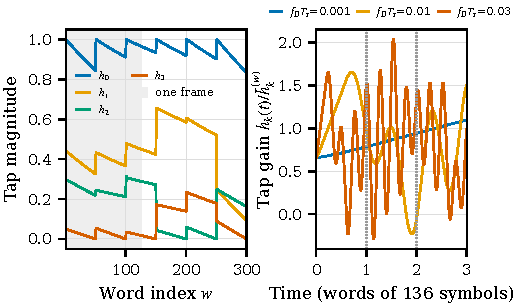
\includegraphics[width=\columnwidth]{channel.pdf}
\caption{Channels. (a) COST~2100 tap magnitudes per word; the shaded region is the 125-word frame used for evaluation. (b) One realization of the fast-fading tap gain over three words for three Doppler values (dotted lines: word boundaries).}
\label{fig:channel}
\end{figure}

\subsection{Complex QPSK channel}
For Section~\ref{sec:qpsk}, QPSK symbols pass through $L=3$ complex Rayleigh taps with an exponential power-delay profile (power ratio 0.5 per tap, unit total power). The taps evolve from word to word as a first-order autoregressive process with correlation 0.99, or, in the fast-fading variant, as complex Jakes processes. Words carry 120 symbols between known start and end symbols; a frame has one pilot word and 24 data words. The trellis has $M^{L-1}=16$ states and $M^L=64$ branches.

\section{Receivers}\label{sec:receivers}
All receivers share the structure of Fig.~\ref{fig:system}: one Viterbi recursion over the 16-state trellis, an RS decoder, and a gate that decides which decoded words are used for adaptation (Section~\ref{sec:protocol}). They differ only in the branch metric $\ell_t(x)$ and in the rule that updates it from pilots and accepted words. Table~\ref{tab:receivers} summarizes them.

\begin{figure}[t]
\centering
% Receiver block diagram: every receiver shares the trellis, decoder and gate;
% only the branch-metric block and its update rule differ.
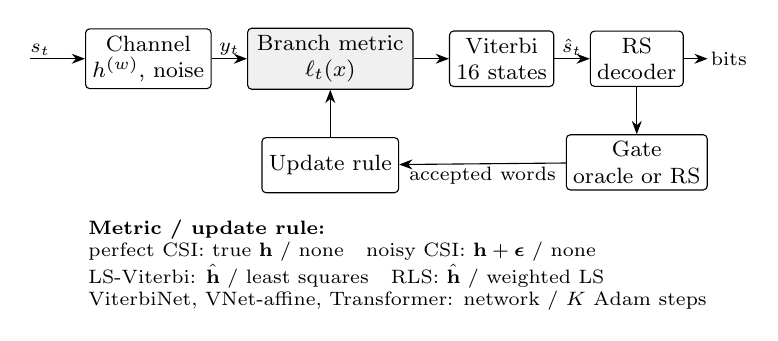
\begin{tikzpicture}[
  font=\footnotesize, >=Stealth, node distance=4mm and 4.5mm,
  blk/.style={draw, rounded corners=1.5pt, minimum height=7mm, align=center, inner sep=2.5pt, fill=white},
  metric/.style={blk, fill=black!6, minimum width=21mm},
  lbl/.style={font=\scriptsize, align=center, inner sep=1pt}]
\node[blk] (ch) {Channel\\$h^{(w)}$, noise};
\node[metric, right=of ch] (met) {Branch metric\\$\ell_t(x)$};
\node[blk, right=of met] (vit) {Viterbi\\16 states};
\node[blk, right=of vit] (rs) {RS\\decoder};
\node[blk, below=6mm of rs] (gate) {Gate\\oracle or RS};
\node[blk, below=6mm of met] (upd) {Update rule};
\draw[->] ([xshift=-7mm]ch.west) node[lbl, above right=0pt and -1pt] {$s_t$} -- (ch);
\draw[->] (ch) -- node[lbl, above] {$y_t$} (met);
\draw[->] (met) -- (vit);
\draw[->] (vit) -- node[lbl, above] {$\hat s_t$} (rs);
\draw[->] (rs) -- ++(9mm,0) node[lbl, right] {bits};
\draw[->] (rs) -- (gate);
\draw[->] (gate) -- node[lbl, below] {accepted words} (upd);
\draw[->] (upd) -- (met);
\node[lbl, anchor=north west, align=left] at ([yshift=-3mm]ch.south west |- upd.south) {
  \textbf{Metric / update rule:}\\
  perfect CSI: true $\mathbf h$ / none\quad noisy CSI: $\mathbf h+\boldsymbol\epsilon$ / none\\
  LS-Viterbi: $\hat{\mathbf h}$ / least squares\quad RLS: $\hat{\mathbf h}$ / weighted LS\\
  ViterbiNet, VNet-affine, Transformer: network / $K$ Adam steps};
\end{tikzpicture}

\caption{Common receiver structure. Only the shaded branch-metric block and its update rule differ between receivers; every adaptive receiver adapts on the same pilots and on the words its own decisions pass through the same gate.}
\label{fig:system}
\end{figure}

\begin{table}[t]
\centering
\caption{Receivers compared (BPSK, $L=4$, $T=136$ samples per word).}
\label{tab:receivers}
\setlength{\tabcolsep}{2.5pt}
\footnotesize
\resizebox{\columnwidth}{!}{%
\begin{tabular}{@{}llrll@{}}
\toprule
Receiver & Branch metric & Param. & Side information & Update per accepted word\\
\midrule
Perfect CSI & Gaussian, true $\mathbf h$ & -- & true taps & none\\
Noisy CSI & Gaussian, $\mathbf h+\boldsymbol\epsilon$ & -- & corrupted taps & none\\
LS-Viterbi & Gaussian, $\hat{\mathbf h}$ & 4 & pilots, accepted words & one LS solve\\
RLS & Gaussian, $\hat{\mathbf h}$ & 4 & pilots, accepted words & weighted LS\\
PSP-LMS & Gaussian, per survivor & $4\times16$ & pilots, own survivors & LMS per symbol\\
ViterbiNet & MLP $1{\to}100{\to}58{\to}16$ & 7,002 & pilots, accepted words & $K$ Adam steps\\
VNet-affine & $\mathbf a y_t+\mathbf b$ & 32 & pilots, accepted words & $K$ Adam steps\\
Transformer V2--V4, ViT & attention, 4-sample window & $\approx$7,000 & pilots, accepted words & $K$ Adam steps\\
\bottomrule
\end{tabular}}
\end{table}

\subsection{Classical receivers}
\emph{Perfect CSI:} $\ell_t(x)=-(y_t-\mathbf h^{\mathsf T}\mathbf s(x))^2/2$ with the true taps (the bound).

\emph{Noisy CSI:} the same metric with taps $1,\dots,L-1$ perturbed by Gaussian noise of standard deviation $\rho$ times the RMS tap magnitude, $\rho\in\{0.25,0.5,0.75,1\}$. This is the CSI-uncertainty baseline of~\cite{shlezinger2020viterbinet}.

\emph{LS-Viterbi (matched information):} the metric uses $\hat{\mathbf h}=\arg\min_{\mathbf h}\sum_t\big(y_t-\mathbf h^{\mathsf T}\mathbf s(x_t)\big)^2$, recomputed on each pilot and on each data word accepted by the gate, with that word's labels. The learned receivers apply the same acceptance and labeling rule to their own decisions.

\emph{LS with forgetting (RLS):} $\hat{\mathbf h}=\mathbf R^{-1}\mathbf r$ with $\mathbf R\leftarrow\lambda\mathbf R+\mathbf X^{\mathsf T}\mathbf X$ and $\mathbf r\leftarrow\lambda\mathbf r+\mathbf X^{\mathsf T}\mathbf y$ over accepted words ($\lambda=0.8$ unless stated), i.e., exponentially weighted LS~\cite{haykin2014adaptive} with an effective memory of $1/(1-\lambda)$ words.

\emph{PSP-LMS:} each survivor carries its own tap estimate, updated by least mean squares along its own path at every trellis step~\cite{raheli1995psp} (step size $\mu=0.01$ unless stated).

\subsection{Learned receivers}
\emph{ViterbiNet:} a fully connected network $1\to100\to58\to16$ (sigmoid, then ReLU; 7,002 parameters) maps $y_t$ to 16 state scores, trained with cross-entropy against the true state. The original uses hidden widths 100 and 50~\cite{shlezinger2020viterbinet}; 58 is this study's implementation choice, which brings the parameter count to that of the attention-based metrics below (about 7,000). Offline training uses 25 minibatches of 300 words with Adam~\cite{kingma2015adam} (learning rate $10^{-3}$); online, $K$ Adam updates are taken on each pilot and each accepted data word, each on the whole word ($K=200$ by default, the number of updates used in~\cite{raviv2023online}, there with mini-batches of 64).

\emph{VNet topologies:} the same pipeline with hidden widths from 4 to 64, two-layer variants, and no hidden layer. The last, VNet-affine, computes $\mathbf a y_t+\mathbf b\in\mathbb R^{16}$ (32 parameters).

\emph{Transformer metrics} (all about 7,000 parameters, window of 4 samples, model width 16): the original encoder with 8 heads; V2 with 2 heads (head width 8) and sinusoidal positions; V3, which replaces the linear embedding with an MLP; V4, an MLP feature extractor, one attention layer, and an MLP head; and ViT variants that treat non-overlapping or overlapping 4-sample patches as tokens~\cite{vaswani2017attention,dosovitskiy2021vit}. All output 16 state scores for the same trellis.

\subsection{QPSK receivers}
\emph{Free per-branch metrics} extend ViterbiNet directly: an affine map (192 parameters) or MLP (9,934 parameters) from $(\Re y_t,\Im y_t)$ to the 64 branch scores. \emph{Tied metrics} constrain the 64 branch means to $\mu_c=\sum_k h_k s_k(c)$ with $L$ learnable complex taps and a learnable scale (7 parameters), optionally adding a shared residual MLP applied to $y_t-\mu_c$ (88 parameters, initialized to zero). \emph{Symbol classifiers} skip the trellis and map a window of received samples to 4 classes: a free linear map (44 parameters), an MLP (948), or an equalizer-structured classifier $z=\mathbf w^{\mathsf H}\mathbf y+b$ with scores $a\,\Re(c_m^* z)$ (21 parameters, 9-sample window). Classical references are LS-Viterbi and a linear equalizer with MMSE weights from the true taps or LS weights re-fitted on its own decisions.

\section{Analysis}\label{sec:analysis}
\subsection{The affine metric contains the ML metric}
\begin{proposition}\label{prop:affine}
For channel \eqref{eq:channel} with known taps and equiprobable states, the posterior logits of the state given one sample are affine in $y_t$: $\log p(x\,|\,y_t)=(\mu_x/\sigma^2)\,y_t-\mu_x^2/(2\sigma^2)+c(y_t)$ with $\mu_x=\mathbf h^{\mathsf T}\mathbf s(x)$. Hence (i) the Bayes-optimal cross-entropy classifier of $x_t$ from $y_t$ lies in the affine family, and (ii) using its logits as branch metrics yields exactly the maximum-likelihood Viterbi decisions.
\end{proposition}
\begin{proof}
$\log p(y_t|x)=-(y_t-\mu_x)^2/(2\sigma^2)+\text{const}$ and $\log p(x)$ is constant, so Bayes' rule gives the stated form with $c(y_t)=-y_t^2/(2\sigma^2)-\log\sum_{x'}p(y_t|x')+\text{const}$. The minimizer of the expected cross-entropy is the true posterior, which is affine up to $c(y_t)$; since softmax is invariant to the state-independent $c(y_t)$, an affine layer attains it. For (ii), $c(y_t)$ adds the same amount to every branch at time $t$, so it changes no comparison in the add-compare-select recursion, and the remaining terms are the Gaussian branch metric up to scale.
\end{proof}
Proposition~\ref{prop:affine} explains why VNet-affine can match a much larger network on this channel: the extra capacity has nothing to represent. It also shows how over-parameterized the affine metric still is: its 32 parameters describe 16 means $\mu_x$ that are fixed by 4 taps. It does not imply that 32 parameters suffice when the noise is non-Gaussian or the channel is nonlinear.

\subsection{Estimation loss of LS-Viterbi}
Let $\hat{\mathbf h}$ be the LS estimate from one word of $T$ samples with correct labels, with noise independent of the samples it is later used on and taps unchanged between estimation and detection. Its error has covariance $\sigma^2(\mathbf X^{\mathsf T}\mathbf X)^{-1}$, so the residual $y_t-\hat{\mathbf h}^{\mathsf T}\mathbf s(x)$ seen by the metric of state $x$ has variance $\sigma^2\big(1+\mathbf s(x)^{\mathsf T}(\mathbf X^{\mathsf T}\mathbf X)^{-1}\mathbf s(x)\big)$. If the shifted-symbol columns of $\mathbf X$ are nearly orthogonal, $\mathbf X^{\mathsf T}\mathbf X\approx T\mathbf I_L$ and the excess is $L/T$. This is an assumption about the training words, not a general LS result, so we checked it for our RS-coded words: averaged over 2,000 random words and the 16 states, $\mathbf s^{\mathsf T}(\mathbf X^{\mathsf T}\mathbf X)^{-1}\mathbf s=0.0301$ against $L/T=0.0294$, and the median condition number of $\mathbf X^{\mathsf T}\mathbf X/T$ is 1.39 (seeded script \texttt{experiments/ls\_loss\_check.py}). Reading this variance increase as an SNR shift is a heuristic rather than a result about sequence errors: to first order LS-Viterbi behaves like the perfect-CSI receiver at an SNR lower by
\begin{equation}\label{eq:loss}
\Delta\approx10\log_{10}\!\left(1+\frac{L}{T}\right)\ \text{dB}=0.126\ \text{dB}\quad(L=4,\ T=136),
\end{equation}
or 0.129~dB with the exact average for the coded words. Shifting the measured perfect-CSI curve by $\Delta$ predicts SER ratios of 1.03, 1.07, 1.16, and 1.27 at 4, 7, 10, and 12~dB; we measure 1.04, 1.06, 1.13, and 1.30 (Fig.~\ref{fig:gap}). At 13--14~dB the prediction (1.31--1.49) slightly exceeds the measurement (1.22--1.25); there the 14~dB point rests on 4 LS bit errors in two repetitions, and the prediction interpolates a perfect-CSI curve that falls by an order of magnitude per dB. The prediction ignores label errors in accepted words and the jumps of Fig.~\ref{fig:channel}a. The measurements are compatible with it, but this agreement does not separate those effects from estimation noise, so we do not attribute the remaining gap to any one of them.

\subsection{Complexity}
For a word of $T$ samples, the trellis costs $O(T\,2^{L+1})$ add-compare-select operations for every receiver. A per-sample metric with $P$ parameters adds about $TP$ multiply-accumulates for the forward pass and $3KTP$ for $K$ adaptation steps (forward and backward), while LS re-estimation costs $O(TL^2+L^3)$, i.e., about $2{,}200$ multiply-accumulates for $T=136$ and $L=4$, fewer than the 7,002-parameter network spends on a single sample. Fig.~\ref{fig:complexity} extends these counts to other memories: the ViterbiNet output layer grows as $2^L$ like the trellis, so learned adaptation stays three to five orders of magnitude above the trellis, while LS re-estimation stays below the trellis for every $L$. Operation counts are the platform-independent measure; measured latency (Section~\ref{sec:latency}) is instead dominated by the trellis, because our trellis is a sequential loop of 136 interpreted steps while the network runs as vectorized kernels.

\begin{figure}[t]
\centering
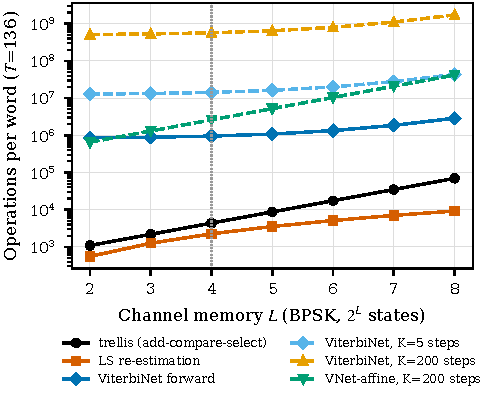
\includegraphics[width=\columnwidth]{complexity.pdf}
\caption{Operations per 136-sample word vs.\ channel memory (BPSK). Network costs scale the $1{\to}100{\to}58{\to}2^L$ ViterbiNet and the $2\cdot2^L$-parameter affine metric; adaptation counts forward and backward passes. Dotted line: $L=4$ used in this paper.}
\label{fig:complexity}
\end{figure}

\section{Evaluation Protocol}\label{sec:protocol}
\emph{Matched information and the adaptation gate.} Every receiver sees the same pilot words (one in every 25 words), and every adaptive receiver uses the same acceptance and labeling rule, applied to its own decisions. We keep the gate of the code base this study builds on: a data word is used for adaptation if the SER of its RS-decoded bits is at most 0.02, with the RS re-encoded word as labels when that SER is zero and the detector's hard decisions otherwise. Computing that SER requires the transmitted bits, so this gate is an oracle, not a receiver function; it is applied identically to every adaptive receiver. We also evaluate an implementable gate that uses no ground truth: accept a word when the re-encoded decoded word differs from the hard decisions in at most one RS symbol (bounded-distance decoding with two parity symbols) and adapt on the re-encoded word (Section~\ref{sec:gate}). This follows the labeling of ViterbiNet's published rule~\cite[Alg.~2]{shlezinger2020viterbinet}, which retrains only when the estimated number of decoding errors is below 2\%, assuming a reliable error estimate such as an error-detection code provides, and always retrains on the re-encoded word. The online meta-learning study~\cite{raviv2023online} implements this rule as a normalized Hamming distance below 0.02 between the re-encoded word and the hard decisions, a receiver-side test close to our RS gate. The oracle gate of our code base departs from both by using raw hard decisions when the decoded SER is nonzero.

\emph{Monte Carlo.} A repetition draws fresh bits and noise for one frame; the SER is computed on the RS-decoded information bits of the 120 data words (14,400 bits per repetition). Learned receivers use 20--50 repetitions per SNR point; the perfect-CSI and LS receivers use at least 100 (up to $10^4$ and $10^3$), with the count set from a predicted SER to target about 100 errors. The simulator's stored average also counts the five pilot words of a frame as error-free; we remove them by scaling it by 125/120. Results are reported from 0 to 14~dB; figures extend to 15~dB, where zero-error points are drawn as the one-sided 95\% bound $3/N$ for $N$ evaluated bits. At 14~dB the SER of ViterbiNet ($K=5$ and 200) and VNet-affine rests on 4--9 bit errors and that of LS-Viterbi on 4; the errors cluster in one or two repetitions, so a Poisson interval (0.3--2.6 times the estimate for 4 errors) and the $3/N$ bound treat them as more independent than they are. Ratios there are indicative only.

\emph{Shared draws and paired comparisons.} The perfect-CSI, LS-Viterbi, ViterbiNet ($K=5$), and VNet-affine receivers read repetition $r<200$ from a shared cache of generated (bits, noise) draws, so their first repetitions are paired; their per-repetition SERs are positively correlated (median $\rho\approx0.5$), as shared draws imply. We report paired differences over the shared repetitions (at most 200), with pointwise paired Student-$t$ 95\% intervals. The $K=200$ ViterbiNet and Transformer sweeps ran with the same code on separate GPU machines with independent draws, and the noisy-CSI sweeps used a separate cache; comparisons against them are unpaired.

\emph{Provenance.} All reported points were generated after we corrected a data-cache defect that had replayed one draw across all repetitions of a point; results collected before the fix were discarded. Every nonzero BPSK point used here (105 points, 0--14~dB) shows repetition-to-repetition variance (standard deviation at least 1.9\% of the mean), which the defect would have made zero. Architecture and topology studies at 7~dB use 20 repetitions each and report 95\% confidence intervals. In the fast-fading study, evaluation data are seeded per repetition, so all receivers see identical transmissions and differences are paired. QPSK points average 64 frames of 24 data words (184,320 symbols).

\emph{Training data.} Offline training of the learned receivers uses words drawn from the same COST~2100 tap sequence used for evaluation. This favors the learned receivers and makes the comparison conservative.

\emph{Hardware.} Latency is measured on a single CPU thread as the median of repeated runs on one 136-sample word. The $K=200$ ViterbiNet and Transformer SNR sweeps were run with the same code on separate GPU machines.

\section{Results}
\subsection{BPSK: matched-information baseline}\label{sec:bpsk}
Fig.~\ref{fig:snr} and Table~\ref{tab:bpsk} report SER versus SNR. In point estimate, LS-Viterbi has the lowest SER of all no-CSI receivers at every SNR from 0 to 14~dB, and it stays within about 3--30\% of the perfect-CSI SER: \serlsseven\ versus \sercsiseven\ at 7~dB, \serlstwelve\ versus \sercsitwelve\ at 12~dB, and \serlsfourteen\ versus \sercsifourteen\ at 14~dB. Relative to ViterbiNet with its default adaptation, LS-Viterbi has 1.3 times lower SER at 7~dB, 9.8 times at 12~dB, and 45 times at 14~dB. With $K=5$ the ratios are 1.07, 1.7, and 20. On the shared draws (Table~\ref{tab:paired}), LS-Viterbi is significantly better than ViterbiNet with $K=5$ at 1, 6, 7, and 9--12~dB and than VNet-affine at 0, 2--7, and 11~dB, and never significantly worse in any available paired comparison; at 13--14~dB the paired differences are not resolved, so the high-SNR ranking is a point-estimate ranking only.

Fig.~\ref{fig:gap} divides every curve by the perfect-CSI SER. Up to 6~dB every no-CSI adaptive receiver is within 1.5 times the bound, and the choice of receiver matters little. The curves separate as the SNR grows: the gap of LS-Viterbi stays flat at 1.0--1.3, as~\eqref{eq:loss} predicts, whereas ViterbiNet with $K=5$ and VNet-affine grow to 1.9--4 times at 12--13~dB and about 25 times at 14~dB, the default ViterbiNet to 13--56 times at 12--14~dB, and the Transformer to 270 times at 14~dB. A learned metric fitted by stochastic gradient updates carries an error floor that is invisible at low SNR and dominant at high SNR; one LS solve does not.

\begin{figure}[t]
\centering
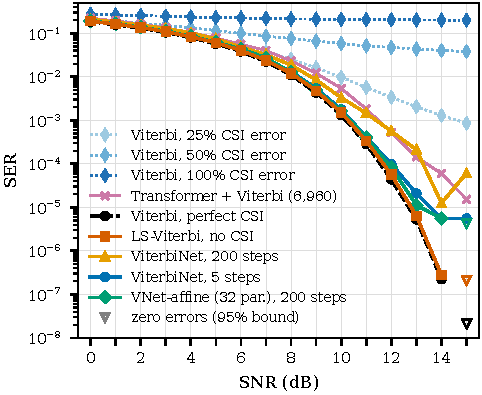
\includegraphics[width=\columnwidth]{ser_snr_journal.pdf}
\caption{BPSK SER vs.\ SNR. LS-Viterbi uses the same pilots and acceptance rule as the learned receivers, applied to its own decisions; noisy-CSI curves perturb the taps by a fixed fraction. Hollow triangles: no errors observed (95\% upper bound).}
\label{fig:snr}
\end{figure}

\begin{table}[t]
\centering
\caption{BPSK SER of the RS-decoded bits.}
\label{tab:bpsk}
\setlength{\tabcolsep}{2.5pt}
\footnotesize
\begin{tabular}{@{}lrccccc@{}}
\toprule
Receiver & Param. & 0 dB & 7 dB & 10 dB & 12 dB & 14 dB\\
\midrule
Viterbi, perfect CSI & -- & \sercsizero & \sercsiseven & \sercsiten & \sercsitwelve & \sercsifourteen\\
Viterbi, 25\% CSI error & -- & \sercsitwentyfivezero & \sercsitwentyfiveseven & \sercsitwentyfiveten & \sercsitwentyfivetwelve & \sercsitwentyfivefourteen\\
LS-Viterbi (no CSI) & 4 & \serlszero & \serlsseven & \serlsten & \serlstwelve & \serlsfourteen\\
ViterbiNet, $K{=}200$ & 7,002 & \servnetzero & \servnetseven & \servnetten & \servnettwelve & \servnetfourteen\\
ViterbiNet, $K{=}5$ & 7,002 & \servnetfivezero & \servnetfiveseven & \servnetfiveten & \servnetfivetwelve & \servnetfivefourteen\\
VNet-affine, $K{=}200$ & 32 & \seraffinezero & \seraffineseven & \seraffineten & \seraffinetwelve & \seraffinefourteen\\
Transformer, $K{=}200$ & 6,960 & \sertransformerzero & \sertransformerseven & \sertransformerten & \sertransformertwelve & \sertransformerfourteen\\
\bottomrule
\end{tabular}
\end{table}

\begin{table}[t]
\centering
\caption{Paired SER differences, LS-Viterbi minus learned receiver, over the Monte Carlo repetitions both evaluated on the same draws (mean $\pm$ pointwise paired Student-$t$ 95\% interval; $^{*}$: interval excludes zero; negative: LS-Viterbi better; --: missing or incomplete per-repetition record for that point).}
\label{tab:paired}
\setlength{\tabcolsep}{3pt}
\footnotesize
\resizebox{\columnwidth}{!}{%
\begin{tabular}{@{}rccr@{}}
\toprule
SNR (dB) & vs.\ ViterbiNet, $K{=}5$ & vs.\ VNet-affine & Reps\\
\midrule
0 & $-1.6\e{-3}\pm1.9\e{-3}$ & $-2.4\e{-3}\pm1.9\e{-3}$$^{*}$ & 20 \\
1 & $-2.6\e{-3}\pm2.2\e{-3}$$^{*}$ & $-1.4\e{-3}\pm1.7\e{-3}$ & 20 \\
2 & $-7.5\e{-4}\pm1.4\e{-3}$ & $-1.9\e{-3}\pm1.5\e{-3}$$^{*}$ & 20 \\
3 & $-1.4\e{-3}\pm1.5\e{-3}$ & $-1.9\e{-3}\pm1.7\e{-3}$$^{*}$ & 20 \\
4 & $-7.6\e{-4}\pm1.2\e{-3}$ & $-2.2\e{-3}\pm1.4\e{-3}$$^{*}$ & 20 \\
5 & -- & $-2.6\e{-3}\pm1.4\e{-3}$$^{*}$ & 20 \\
6 & $-1.8\e{-3}\pm1.0\e{-3}$$^{*}$ & $-3.8\e{-3}\pm2.1\e{-3}$$^{*}$ & 20 \\
7 & $-1.9\e{-3}\pm1.0\e{-3}$$^{*}$ & $-3.6\e{-3}\pm3.0\e{-3}$$^{*}$ & 20 \\
8 & -- & $-4.6\e{-4}\pm1.2\e{-3}$ & 20 \\
9 & $-7.8\e{-4}\pm4.6\e{-4}$$^{*}$ & $-3.9\e{-4}\pm5.5\e{-4}$ & 21 \\
10 & $-2.5\e{-4}\pm1.2\e{-4}$$^{*}$ & $-1.2\e{-4}\pm1.5\e{-4}$ & 50 \\
11 & $-9.3\e{-5}\pm6.6\e{-5}$$^{*}$ & $-8.5\e{-5}\pm7.2\e{-5}$$^{*}$ & 50 \\
12 & $-5.0\e{-5}\pm3.7\e{-5}$$^{*}$ & $-3.3\e{-5}\pm3.5\e{-5}$ & 50 \\
13 & $-2.8\e{-6}\pm1.6\e{-5}$ & $+6.9\e{-6}\pm1.1\e{-5}$ & 50 \\
14 & $-2.8\e{-6}\pm1.2\e{-5}$ & $-2.8\e{-6}\pm1.2\e{-5}$ & 50 \\
\bottomrule

\end{tabular}}
\end{table}

\begin{figure}[t]
\centering
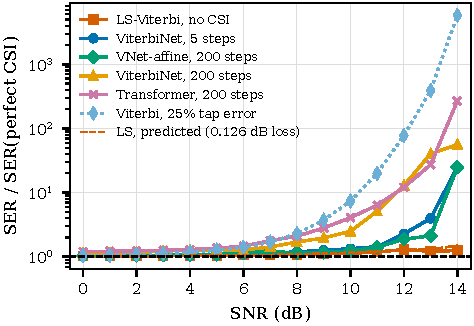
\includegraphics[width=\columnwidth]{gap_ratio.pdf}
\caption{SER relative to the perfect-CSI Viterbi detector, 0--14~dB. Dashed red: LS-Viterbi predicted from~\eqref{eq:loss}. At 14~dB the ViterbiNet and VNet-affine points rest on 4--9 bit errors, clustered in few repetitions.}
\label{fig:gap}
\end{figure}

\subsection{An implementable adaptation gate}\label{sec:gate}
The results above use the oracle gate (Section~\ref{sec:protocol}). Table~\ref{tab:gate} repeats four adaptive receivers with the implementable RS gate, evaluating the same repetitions, so each receiver's two rows are paired. Each receiver starts from its sweep's offline weights, except that the $K=200$ ViterbiNet runs start from the offline weights of the $K=5$ sweep, not those of the separately trained $K=200$ sweep; its rows therefore compare the two gates, not the main $K=200$ results. The implementable gate is stricter at low SNR: at 7~dB it accepts 21--33\% of data words against 30--44\% for the oracle gate. It is also cleaner, because it always adapts on a codeword: 15--22\% of the accepted words carry any label error, against 37--46\% for the oracle gate, whose labels are raw hard decisions whenever the decoded SER is nonzero. At 10 and 12~dB both gates accept most words (83--100\%), and both label errors and differences shrink. LS-Viterbi keeps the lowest point-estimate SER under both gates at all three SNRs. The gates are not equivalent, however: of the twelve paired RS-minus-oracle differences in Table~\ref{tab:gate}, one is significant, VNet-affine at 7~dB ($+7.7\e{-4}\pm5.6\e{-4}$), and the others are not resolved. We therefore claim only that the ranking at the top is unchanged at the SNRs tested, not that the two gates give the same SERs.

\begin{table}[t]
\centering
\caption{Oracle vs.\ implementable (RS) adaptation gate on the same draws: SER, fraction of data words accepted, fraction of accepted words with wrong labels, and paired SER difference RS minus oracle (pointwise Student-$t$ 95\% interval; $^{*}$: excludes zero).}
\label{tab:gate}
\setlength{\tabcolsep}{2.5pt}
\footnotesize
\resizebox{\columnwidth}{!}{%
\begin{tabular}{@{}rlccccccc@{}}
\toprule
& & \multicolumn{2}{c}{SER} & \multicolumn{2}{c}{Accepted} & \multicolumn{2}{c}{Wrong labels} & SER diff.\\
\cmidrule(lr){3-4}\cmidrule(lr){5-6}\cmidrule(lr){7-8}\cmidrule(l){9-9}
SNR & Receiver & oracle & RS & oracle & RS & oracle & RS & RS$-$oracle\\
\midrule
7 & LS-Viterbi & $2.4\e{-2}$ & $2.4\e{-2}$ & 0.44 & 0.33 & 0.37 & 0.149 & $+1.2\e{-4}\pm3.4\e{-4}$ \\
 & ViterbiNet $K{=}5$ & $2.5\e{-2}$ & $2.5\e{-2}$ & 0.42 & 0.30 & 0.38 & 0.165 & $+1.8\e{-4}\pm5.6\e{-4}$ \\
 & VNet-affine $K{=}200$ & $2.5\e{-2}$ & $2.6\e{-2}$ & 0.43 & 0.29 & 0.38 & 0.164 & $+7.7\e{-4}\pm5.6\e{-4}$$^{*}$ \\
 & ViterbiNet $K{=}200$ & $3.2\e{-2}$ & $3.2\e{-2}$ & 0.30 & 0.21 & 0.46 & 0.219 & $-1.7\e{-4}\pm2.0\e{-3}$ \\
10 & LS-Viterbi & $1.5\e{-3}$ & $1.6\e{-3}$ & 0.97 & 0.93 & 0.04 & 0.003 & $+1.7\e{-5}\pm5.4\e{-5}$ \\
 & ViterbiNet $K{=}5$ & $1.8\e{-3}$ & $1.7\e{-3}$ & 0.96 & 0.93 & 0.04 & 0.004 & $-1.0\e{-4}\pm1.8\e{-4}$ \\
 & VNet-affine $K{=}200$ & $1.7\e{-3}$ & $1.7\e{-3}$ & 0.97 & 0.93 & 0.05 & 0.005 & $-2.4\e{-5}\pm1.1\e{-4}$ \\
 & ViterbiNet $K{=}200$ & $4.1\e{-3}$ & $4.4\e{-3}$ & 0.91 & 0.83 & 0.09 & 0.010 & $+3.0\e{-4}\pm1.1\e{-3}$ \\
12 & LS-Viterbi & $4.6\e{-5}$ & $4.6\e{-5}$ & 1.00 & 1.00 & 0.00 & 0.001 & 0 \\
 & ViterbiNet $K{=}5$ & $1.1\e{-4}$ & $1.0\e{-4}$ & 1.00 & 1.00 & 0.00 & 0.001 & $-6.9\e{-6}\pm5.2\e{-5}$ \\
 & VNet-affine $K{=}200$ & $7.9\e{-5}$ & $7.6\e{-5}$ & 1.00 & 1.00 & 0.00 & 0.000 & $-2.3\e{-6}\pm4.7\e{-6}$ \\
 & ViterbiNet $K{=}200$ & $6.7\e{-4}$ & $7.2\e{-4}$ & 0.98 & 0.97 & 0.02 & 0.003 & $+4.6\e{-5}\pm1.9\e{-4}$ \\
\bottomrule

\end{tabular}}
\end{table}

\subsection{The noisy-CSI baseline}\label{sec:csi}
Fig.~\ref{fig:csi} illustrates the uncertain-CSI comparison in our implementation. With 25\% tap error the Viterbi detector improves only slowly with SNR and reaches $1.3\e{-3}$ at 14~dB, 5,800 times the perfect-CSI reference (Fig.~\ref{fig:gap}); at 50--100\% error it is flat at 0.04--0.2. ViterbiNet beats these fixed-estimate curves from 6~dB on, consistent with the robustness comparison in~\cite{shlezinger2020viterbinet}. We additionally let the classical receiver adapt: LS-Viterbi estimates four taps from the pilots and accepted decisions with one least-squares solve per accepted word. The tested learned receiver then has no established SER advantage over this adaptive baseline.

\begin{figure}[t]
\centering
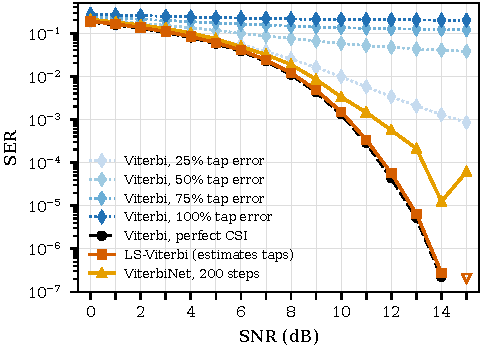
\includegraphics[width=\columnwidth]{csi_uncertainty.pdf}
\caption{The CSI-uncertainty baseline: Viterbi with taps perturbed by 25--100\% of their RMS magnitude, against the perfect-CSI and LS-Viterbi receivers and ViterbiNet.}
\label{fig:csi}
\end{figure}

\subsection{Online adaptation budget}\label{sec:adapt}
Fig.~\ref{fig:steps} sweeps the number of online steps $K$ at 7~dB. For the 7,002-parameter network the SER is lowest at $K=5$ (0.0249) and rises monotonically to 0.0315 at $K=200$. Without adaptation it is 0.0340, so a few steps help and many steps overfit: each step fits the same 136-sample word, and after a handful of steps the network starts fitting that word's noise. Over the whole SNR range, $K=5$ has a lower point-estimate SER than $K=200$ at every SNR (Table~\ref{tab:bpsk}, Fig.~\ref{fig:gap}; unpaired, since the $K=200$ sweep used independent draws) while using 40 times fewer adaptation updates.

The affine metric responds oppositely: it needs 50--200 steps to move from the generic offline solution to the frame's channel and reaches 0.0254 at $K=100$--200, statistically tied with the tuned network. Over the range tested its SER kept falling up to $K=100$--200, so we did not observe the overfitting seen for the network. This does not show that a 32-parameter model cannot overfit; in these runs, more update steps were needed to reach its best observed SER.

\begin{figure}[t]
\centering
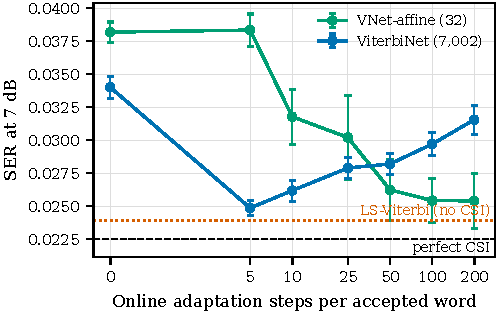
\includegraphics[width=\columnwidth]{online_steps.pdf}
\caption{SER at 7~dB vs.\ online steps per accepted word (25 offline minibatches; bars: 95\% confidence intervals over 20 repetitions).}
\label{fig:steps}
\end{figure}

\subsection{Topology: structure over size}\label{sec:topology}
Fig.~\ref{fig:topology}(a) shows SER against parameter count at the default budget. SER increases with size, from 0.0254 (affine) to 0.0275--0.0290 (4 to 64 hidden units), 0.0299--0.0307 (two hidden layers) and 0.0315 (7,002 parameters). Only the confidence intervals of the smallest networks overlap the affine one. Fig.~\ref{fig:topology}(b) varies the offline budget: from 2 to 25 minibatches the large network stays near 0.031--0.033, whereas the affine metric improves with more offline training. More capacity does not buy accuracy, because the metric the network must represent is quadratic in $y_t$ with four unknowns (Proposition~\ref{prop:affine}).

\begin{figure*}[t]
\centering
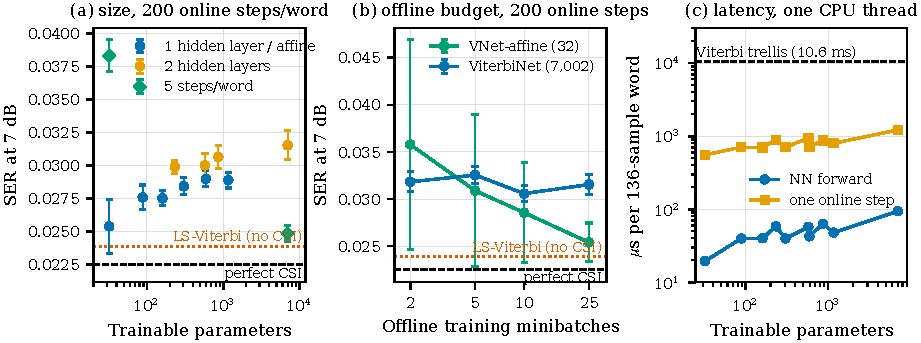
\includegraphics[width=\textwidth]{topology.pdf}
\caption{ViterbiNet topology study at 7~dB. (a) SER vs.\ trainable parameters at 25 offline minibatches and 200 online steps (green: 5 online steps). (b) SER vs.\ offline minibatches. (c) Per-word latency of the network forward pass and one online step; the 16-state trellis costs about 10.6~ms per word for every topology.}
\label{fig:topology}
\end{figure*}

\subsection{Sequence architectures and training budget}\label{sec:arch}
Fig.~\ref{fig:arch} compares metrics of about 7,000 parameters at 7~dB under a training-budget search: starting at 25 offline minibatches, the budget grows by 25 while the SER improves and is then refined by a binary search around the best value, with fixed-budget runs up to 1,000 minibatches. The MLP is best at every budget (0.031--0.033). The best attention-based metric, a ViT with overlapping patches, reaches 0.033 after 250 minibatches; Transformer V2, V3, and V4 stay between 0.037 and 0.041; the original 8-head encoder reaches 0.040; and a ViT with non-overlapping patches fails (0.107), because a 4-sample patch splits the channel memory across tokens. Attention over a 4-sample window adds no information the trellis does not already use, and the extra parameters are spent on mixing that the channel structure makes unnecessary. Over the SNR sweep the Transformer trails LS-Viterbi, ViterbiNet with $K=5$, and VNet-affine at every SNR, and ViterbiNet with $K=200$ everywhere except 12 and 13~dB, where its point estimate is slightly lower (Fig.~\ref{fig:gap}).

\begin{figure}[t]
\centering
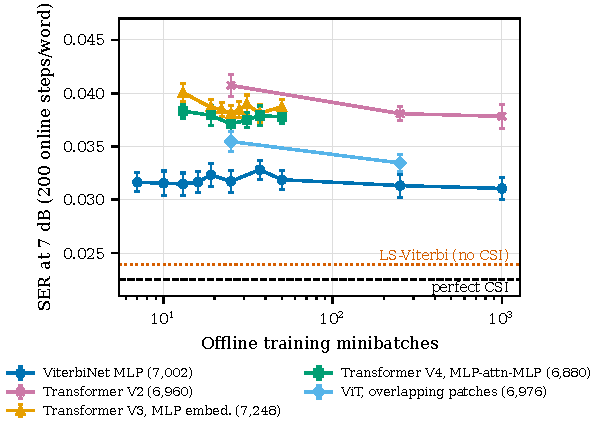
\includegraphics[width=\columnwidth]{architectures.pdf}
\caption{SER at 7~dB vs.\ offline training budget for metrics of about 7,000 parameters (200 online steps; bars: 95\% confidence intervals).}
\label{fig:arch}
\end{figure}

\subsection{Latency, real-time budget, and the accuracy--compute trade-off}\label{sec:latency}
Fig.~\ref{fig:latency} breaks detection latency down on one CPU thread. The 136-step, 16-state trellis costs 11--12~ms per word (81--90~$\mu$s per symbol) for every receiver. The network forward pass adds 0.05~ms (affine), 0.14~ms (ViterbiNet), and 1.4--2.4~ms (attention-based). The difference that matters is adaptation: one online step takes 0.53~ms (affine), 1.0~ms (ViterbiNet), and 4.9--7.3~ms (attention-based).

Fig.~\ref{fig:realtime} adds the adaptation of one accepted word to the detection time and compares the total with the duration of a word at 8~ksymbol/s (0.125~ms per symbol, 17~ms per word). LS-Viterbi needs 11.4~ms (the measured trellis time plus a separately timed 0.02~ms LS solve) and ViterbiNet with $K=5$ 16.8~ms (1.4\% headroom), both inside this measured detection-plus-adaptation budget on a single thread of an interpreted implementation. These are median component timings that exclude RS decoding and gating, so they do not establish a full receiver deadline. VNet-affine with $K=200$ (117~ms), the default ViterbiNet (220~ms), and the Transformers (0.99--1.5~s) exceed it by one to two orders of magnitude and would need batching across words, dedicated hardware, or fewer steps.

Fig.~\ref{fig:pareto} plots SER at 7~dB against adaptation compute per accepted word for every topology and budget. The LS receiver sits at the lower left: 0.02~ms for one solve and an SER below every learned point. Among the learned receivers the Pareto front is formed by ViterbiNet with $K=5$ (5~ms) and the affine metric with $K=200$ (105~ms); the default ViterbiNet (209~ms) is dominated by both, and the Transformers (about 1~s) are dominated by all. A smaller network is therefore not automatically a cheaper receiver: the number of adaptation steps it needs matters as much as its size.

\begin{figure}[t]
\centering
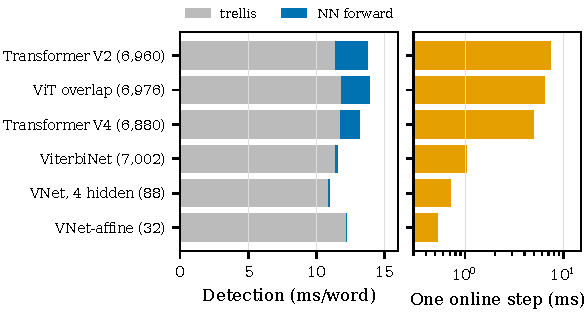
\includegraphics[width=\columnwidth]{latency.pdf}
\caption{Per-word latency on one CPU thread: detection (trellis plus network forward pass) and one online adaptation step.}
\label{fig:latency}
\end{figure}

\begin{figure}[t]
\centering
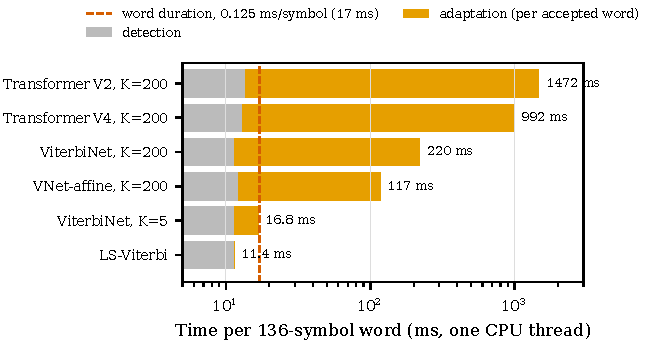
\includegraphics[width=\columnwidth]{realtime.pdf}
\caption{Detection plus adaptation time per accepted 136-symbol word on one CPU thread, against the word duration at 0.125~ms per symbol.}
\label{fig:realtime}
\end{figure}

\begin{figure}[t]
\centering
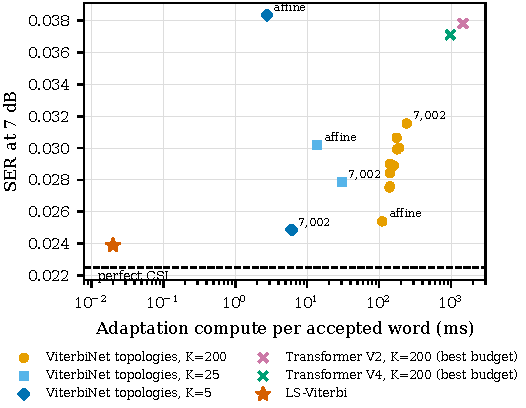
\includegraphics[width=\columnwidth]{pareto.pdf}
\caption{Accuracy vs.\ adaptation compute at 7~dB. Circles, squares, diamonds: ViterbiNet topologies (4 hidden units to 7,002 parameters, and the affine metric) at $K=200$, 25, and 5 online steps. Crosses: Transformers at their best offline budget. Star: LS-Viterbi.}
\label{fig:pareto}
\end{figure}

\subsection{QPSK: tying the branch classes}\label{sec:qpsk}
Fig.~\ref{fig:qpsk} and Table~\ref{tab:qpsk} show the complex QPSK channel from 0 to 14~dB. The free per-branch metrics, the direct extension of ViterbiNet, fail: at 14~dB they reach 0.44 (affine) and 0.57 (MLP), 14 and 18 times the LS-Viterbi SER, and their gap grows with SNR. The tied metric (7 parameters) stays within 1.1--1.8 times LS-Viterbi at every SNR, and the tied metric with a residual MLP (88 parameters) within 1.2--2.9 times except at 14~dB, where it is 2.5 times better ($1.3\e{-2}$ against $3.2\e{-2}$). Neighboring SNR points use independent channel draws and the tracking receivers propagate decision errors, so single points fluctuate; comparisons are meaningful within an SNR point, where all receivers share the draws.

\begin{figure}[t]
\centering
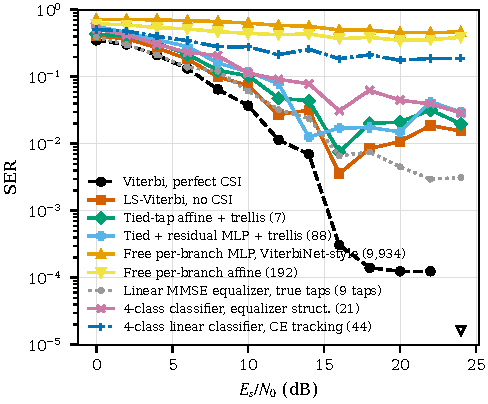
\includegraphics[width=\columnwidth]{qpsk.pdf}
\caption{QPSK, 3 complex taps drifting between words, one 120-symbol pilot per 25 words. Parentheses: trainable parameters.}
\label{fig:qpsk}
\end{figure}

\begin{table}[t]
\centering
\caption{QPSK SER (64 frames $\times$ 24 data words per point).}
\label{tab:qpsk}
\setlength{\tabcolsep}{3pt}
\footnotesize
\resizebox{\columnwidth}{!}{%
\begin{tabular}{@{}lrcccc@{}}
\toprule
Receiver & Param. & 4 dB & 8 dB & 12 dB & 14 dB\\
\midrule
Viterbi, perfect CSI & -- & 0.21 & $6.5\e{-2}$ & $1.1\e{-2}$ & $7.0\e{-3}$\\
LS-Viterbi & -- & 0.27 & 0.10 & $2.7\e{-2}$ & $3.2\e{-2}$\\
Tied affine + trellis & 7 & 0.32 & 0.12 & $4.8\e{-2}$ & $4.4\e{-2}$\\
Tied + residual MLP + trellis & 88 & 0.36 & 0.16 & $7.9\e{-2}$ & $1.3\e{-2}$\\
Free per-branch affine & 192 & 0.54 & 0.47 & 0.43 & 0.44\\
Free per-branch MLP & 9,934 & 0.71 & 0.67 & 0.59 & 0.57\\
4-class linear, CE tracking & 44 & 0.40 & 0.28 & 0.21 & 0.26\\
4-class MLP, CE tracking & 948 & 0.41 & 0.30 & 0.24 & 0.29\\
4-class, equalizer structure & 21 & 0.31 & 0.21 & $9.2\e{-2}$ & $7.9\e{-2}$\\
Linear equalizer, LS weights & -- & 0.30 & 0.20 & $8.8\e{-2}$ & $7.9\e{-2}$\\
Linear MMSE, true taps & -- & 0.21 & 0.12 & $3.2\e{-2}$ & $2.4\e{-2}$\\
\bottomrule
\end{tabular}}
\end{table}

\emph{Why the free metric fails: data, not tracking.} Fig.~\ref{fig:pilot} removes the drift (static channel, 14~dB) and varies the pilot. LS-Viterbi and the tied metric reach $4.5$--$8.4\e{-4}$ with a single 120-symbol pilot word and gain nothing from longer pilots. The free per-branch affine metric stays at 0.24 with one pilot word (0.13 with ten times more training steps); it needs 5 pilot words and 2,000 steps to reach $1.2\e{-3}$, within 2 times of the tied metric, at five times the pilot overhead. The free MLP never goes below 0.10, even with 10 pilot words. The failure is therefore one of data: a 120-symbol pilot visits each of the 64 branches about twice on average, and about 10 branches not at all, so a metric that learns each branch mean separately cannot be trained from one pilot. The tied metric estimates 3 taps from the same 120 symbols and generalizes to every branch, which is why it matches LS-Viterbi with a single pilot.

\begin{figure}[t]
\centering
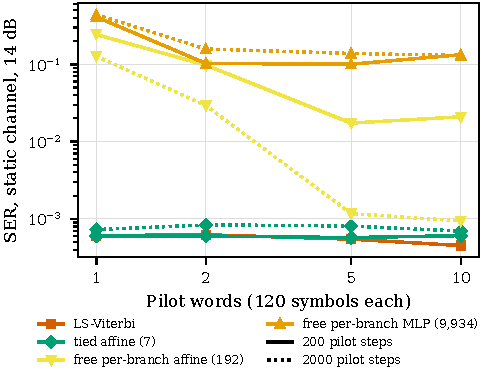
\includegraphics[width=\columnwidth]{qpsk_pilot.pdf}
\caption{QPSK on a static channel at 14~dB: SER vs.\ pilot length with 200 (solid) or 2,000 (dotted) pilot training steps. Parentheses: trainable parameters.}
\label{fig:pilot}
\end{figure}

\emph{Why symbol classifiers need structure.} A free linear or MLP 4-class classifier trained on the pilot and adapted by cross-entropy on its own decisions stays at 0.21--0.29 at 12--14~dB. Fig.~\ref{fig:trace} shows why: its per-word SER climbs from 0.16 to 0.38 across the frame at 12~dB and from 0.10 to 0.28 at 14~dB. Confident decisions produce almost no cross-entropy gradient, so self-training never follows the drifting channel, and a code gate at SER 0.02 would never open. Giving the classifier an equalizer structure and a decision-directed LMS update holds it at 0.07--0.10 across the frame and brings it to $7.9\e{-2}$ at 14~dB, equal to a linear equalizer whose weights are re-fitted by LS on its own decisions (Table~\ref{tab:qpsk}; the two agree within 10\% at every SNR). The trellis receivers degrade across the frame as well, LS-Viterbi from 0.012 to 0.036 and the tied metric from 0.014 to 0.056 at 14~dB, but remain below every symbol classifier.

\begin{figure}[t]
\centering
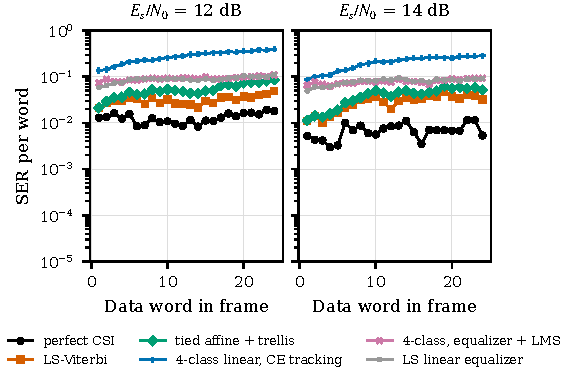
\includegraphics[width=\columnwidth]{qpsk_trace.pdf}
\caption{QPSK per-word SER across the 24 data words of a frame (64 frames; one pilot before word 1). Words without errors are not drawn.}
\label{fig:trace}
\end{figure}

\emph{The window limits linear equalization.} Fig.~\ref{fig:window} varies the equalizer window. With true taps the MMSE equalizer improves from 0.11 (3 samples) to $2.1\e{-2}$ (9) and $1.7\e{-2}$ (15) at 14~dB, still 2.4 times the perfect-CSI trellis. With LS weights fitted on its own decisions it stalls at 0.066--0.069 from 9 samples on, because decision errors bias the fit. The 9-sample window of the equalizer-structured classifier is therefore near the best a decision-directed linear receiver can do, and the remaining gap to the trellis is the cost of symbol-by-symbol detection.

\begin{figure}[t]
\centering
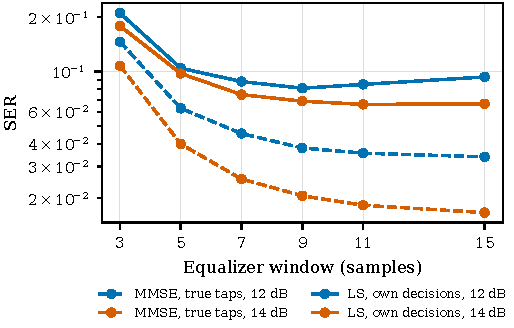
\includegraphics[width=\columnwidth]{qpsk_window.pdf}
\caption{QPSK linear equalizers vs.\ window length: MMSE weights from the true taps (dashed) and LS weights re-fitted on the equalizer's own decisions (solid).}
\label{fig:window}
\end{figure}

\subsection{Fast fading}\label{sec:ff}
Fig.~\ref{fig:ffb} and Table~\ref{tab:ff} show BPSK at 7~dB when the taps vary within the word. Because all receivers see the same transmissions, we report paired differences. At $f_DT_s=0.001$ the learned receivers beat LS-Viterbi on the last accepted word by 0.039 SER and PSP-LMS by 0.017. The source of that advantage is memory rather than tracking: exponentially weighted LS with forgetting factor 0.8 ties VNet-affine up to $f_DT_s=0.01$ and beats it at 0.03, and it is slightly better than ViterbiNet with $K=5$ at $f_DT_s=0.001$ and 0.03. After a deep fade, the last accepted word is a poor estimate of the next one; an estimator that averages over past words, whether by offline training on the channel statistics or by exponential forgetting, is not misled by it. None of the receivers without CSI approaches a genie that knows the per-sample taps, including PSP-LMS, which updates its tap estimates at every trellis step: all sit near 0.14, against 0.07 for the genie.

\begin{figure}[t]
\centering
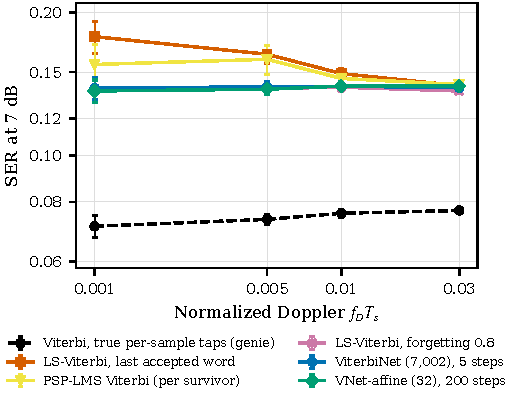
\includegraphics[width=\columnwidth]{fast_fading_bpsk.pdf}
\caption{BPSK SER at 7~dB vs.\ normalized Doppler (Rician $\kappa=3$ Jakes fading within the word; 50 paired repetitions; bars: 95\% confidence intervals).}
\label{fig:ffb}
\end{figure}

\begin{table}[t]
\centering
\caption{Paired SER differences under BPSK fast fading at 7~dB (mean $\pm$ 95\% CI over 50 repetitions; positive: first receiver worse).}
\label{tab:ff}
\setlength{\tabcolsep}{3pt}
\footnotesize
\resizebox{\columnwidth}{!}{%
\begin{tabular}{@{}lcccc@{}}
\toprule
$f_DT_s$ & 0.001 & 0.005 & 0.01 & 0.03\\
\midrule
LS (last word) $-$ ViterbiNet $K{=}5$ & $+.039\pm.011$ & $+.024\pm.006$ & $+.009\pm.003$ & $+.001\pm.002$\\
RLS ($\lambda{=}0.8$) $-$ ViterbiNet $K{=}5$ & $-.002\pm.001$ & $-.001\pm.001$ & $-.001\pm.001$ & $-.002\pm.002$\\
RLS ($\lambda{=}0.8$) $-$ VNet-affine & $+.000\pm.001$ & $+.001\pm.001$ & $-.001\pm.001$ & $-.003\pm.001$\\
\bottomrule
\end{tabular}}
\end{table}

\emph{Sensitivity to the tracker settings.} The classical trackers above use a single step size and forgetting factor. Fig.~\ref{fig:tuning} sweeps both on 20 paired repetitions and reports the difference to VNet-affine on the same draws. PSP-LMS is sensitive to its step size. Its best setting is $\mu=0.01$ at $f_DT_s=0.001$ and $\mu=0.003$ at 0.01 and 0.03; there it is within $0.002$--$0.005$ of VNet-affine at the two higher Doppler values but $0.013\pm0.015$ worse at 0.001, where a per-symbol LMS update is too noisy to beat averaging over words, and $\mu=0.05$ diverges ($+0.09$ to $+0.19$). Exponentially weighted LS is insensitive to its forgetting factor: any memory from 5 to 100 words ($\lambda=0.8$--0.99) ties VNet-affine within $\pm0.002$ at $f_DT_s\le0.01$ and beats it by 0.003--0.004 at 0.03 (95\% CI $\pm0.002$). A memory of two words ($\lambda=0.5$) already recovers most of the gap that LS on the last word leaves ($+0.005$ against $+0.038$ at $f_DT_s=0.001$). Tuning therefore strengthens the conclusion: a classical estimator with memory matches the learned receivers over a wide range of its only parameter, and no setting of either tracker approaches the genie (0.069--0.078).

\begin{figure}[t]
\centering
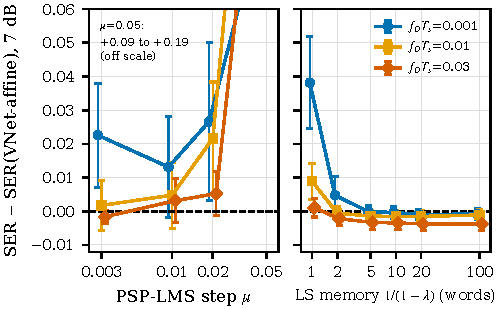
\includegraphics[width=\columnwidth]{tracker_tuning.pdf}
\caption{Classical tracker settings under BPSK fast fading at 7~dB: SER minus that of VNet-affine on the same 20 repetitions (bars: 95\% CI of the paired difference). (a) PSP-LMS step size. (b) LS forgetting factor, as effective memory in words; 1 is LS on the last accepted word.}
\label{fig:tuning}
\end{figure}

The complex QPSK channel is harsher (Fig.~\ref{fig:ffq}), because tap phases rotate. At $f_DT_s=2\times10^{-4}$ (0.02 Doppler cycles per word) the trellis receivers are already 6--8 times worse than the genie at 10~dB and 13--15 times worse at 14~dB, where LS-Viterbi and the tied metric reach 0.099 and 0.101 against $7.7\e{-3}$. At $f_DT_s\ge5\times10^{-4}$ every receiver that estimates one channel per word, learned or classical, trellis or equalizer, falls to 0.56--0.75, near chance (0.75), while the genie stays at $5$--$8\e{-3}$ at 14~dB. The learned and classical receivers fail together and by the same amount, so the limitation is the per-word channel model shared by all of them, not the choice between learning and estimation.
Handling such channels requires tracking within the word, which none of the learned receivers studied here provides.

\begin{figure}[t]
\centering
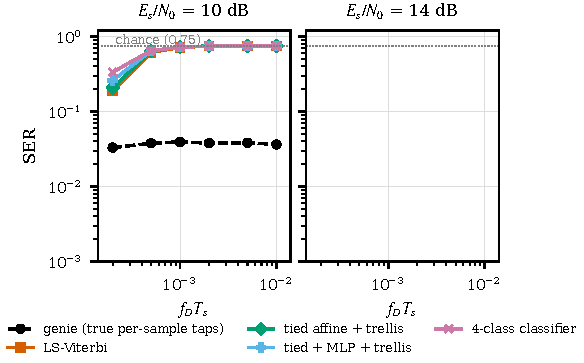
\includegraphics[width=\columnwidth]{fast_fading_qpsk.pdf}
\caption{QPSK SER vs.\ normalized Doppler with complex Jakes taps varying within the word (64 frames per point, identical draws for all receivers).}
\label{fig:ffq}
\end{figure}

\section{Discussion}
\emph{When does learning help?} In the main BPSK SNR sweep, the branch metric is fixed by a linear channel and Gaussian noise: it is quadratic in the received sample, with $L$ unknown taps. A classical receiver that estimates those taps from the same data comes close to the perfect-CSI bound, roughly as the loss~\eqref{eq:loss} predicts. In that sweep, none of the learned receivers had a lower point-estimate SER than LS-Viterbi. Under fast fading, learned receivers beat last-word LS by using channel memory, but not LS with exponential forgetting (Section~\ref{sec:ff}); in that setting, no tested no-CSI receiver approaches the genie. Learning can add value where this model is wrong: nonlinear front ends, impulsive or non-Gaussian noise, or channels without a finite-tap description~\cite{farsad2018neural}. Our results support including a matched-information adaptive classical receiver alongside perfect-, uncertain-, and stale-CSI references when assessing the additional benefit of learning.

\emph{Where the learned receivers lose.} The losses are small at low SNR and grow with SNR (Fig.~\ref{fig:gap}). A metric trained by a few stochastic gradient steps on a noisy target has a residual error that stops mattering only when noise dominates. The same mechanism explains the overfitting of $K=200$ (Fig.~\ref{fig:steps}), the inefficiency of the attention metrics (Fig.~\ref{fig:arch}), and the failure of free per-branch metrics for QPSK (Fig.~\ref{fig:pilot}): every added parameter must be estimated from the same few hundred labeled samples.

\emph{Design guidance.} (i) Compare against a classical receiver that receives the same pilots and acceptance rule, applied to its own decisions. (ii) Tune the online adaptation budget; the right number of steps depends on model size and can differ by two orders of magnitude. (iii) Build the channel structure into the metric: for $M$-ary signalling, tie the $M^L$ branch classes to $L$ taps. (iv) Measure cost end to end against the symbol rate, and count operations as well as time; the adaptation loop, not the network forward pass, sets the cost of a learned receiver, while LS re-estimation costs less than the trellis itself. (v) Under fast fading, evaluate tracking within the word against PSP or exponentially weighted estimators before attributing gains to learning. (vi) Report results where they are statistically supported; above about 14~dB in our setting the learned receivers' SER rests on a handful of errors.

\emph{Limitations.} Our BPSK results use one COST~2100 tap trace, a linear Gaussian channel, and our own implementation of ViterbiNet; the QPSK and fast-fading channels are synthetic. The meta-learning variants of~\cite{raviv2021metaviterbinet,raviv2023online} change how the learned receivers adapt and should be compared against the same baselines. Latency was measured in an interpreted implementation on one CPU thread; absolute numbers and the share of the trellis will change on other platforms, whereas the operation counts of Fig.~\ref{fig:complexity} do not.

\section{Conclusion}
Given the same pilots and acceptance rule, a least-squares Viterbi receiver had the lowest point-estimate SER of all no-CSI receivers in the BPSK SNR sweep from 0 to 14~dB, significantly lower than ViterbiNet with $K=5$ at most SNRs from 6 to 12~dB and never significantly higher in any available paired comparison, with 13--14~dB unresolved. It stayed within about 3--30\% of the perfect-CSI SER, roughly as a simple estimation-loss argument predicts, and needed a single least-squares solve per accepted word to adapt. In the BPSK sweep, the tested learned metrics show no established advantage over LS-Viterbi. Under fast fading, they outperform last-word LS, but exponentially weighted LS matches or improves on their performance. These findings extend the original evaluation with adaptive classical baselines; they do not invalidate the architectural contribution, and meta-learned variants were not tested. Within the learned family, fewer adaptation steps, fewer parameters, and structure tied to the channel model all helped, and attention-based metrics did not. The open problem these experiments expose is tracking within a word under fast fading, where every receiver without CSI, learned or classical, remains far from the bound.

\section*{Data Availability and AI-Use Statement}
Simulation code, raw results, and the scripts that generate every figure and table (\texttt{paper/make\_figures.py}) are available at \url{https://github.com/Gilzuk/viterbinet-revisited} (release \texttt{v1.0-submission}). An AI coding assistant (Claude, Anthropic) was used to write simulation, analysis, and plotting code and to draft the manuscript; the author checked all code, results, and text.

\bibliographystyle{IEEEtran}
\bibliography{../refs}

\end{document}
